\documentclass[11pt]{article}
\usepackage[notes]{la}
\lamodule{1}{8}{Introduction to Linear Transformations}
\laxdoc{1.4}
\laxdoc{1.5}
\laxdoc{1.7}

\begin{document}

\section{Introduction to Linear Transformations}

\begin{guide}
Until now a matrix $A$ was a table of coefficients, and $A\bv{x}=\bv{b}$ was a question to be answered. Turn the equation around: fix $A$ and let $\bv{x}$ vary. Then $\bv{x}\mapsto A\bv{x}$ is a \emph{function} that sends every vector of $\R^n$ to a vector of $\R^m$.
What does such a function do to the plane: to lines, to a grid, to a unit square? Which property of it is so important that it deserves a name? And is every function that sends lines to lines of this kind?
\end{guide}

\textbf{By the end of this section you should be able to:}
\begin{itemize}
  \item describe $\bv{x}\mapsto A\bv{x}$ as a function with a domain, codomain, images and a range, and compute images and preimages;
  \item decide whether a vector lies in the range of a matrix transformation, using row reduction;
  \item state the definition of a linear transformation, test a formula for linearity, and produce a counterexample when it fails;
  \item use $T(\bv{0})=\bv{0}$ and the superposition rule to compute $T$ of a linear combination;
  \item describe geometrically what a linear transformation does to lines, parallelograms and grids;
  \item explain why two inputs share an output exactly when their difference is sent to $\bv{0}$, and how this is the translate theorem of Section~1.5 in new words;
  \item explain what a linear transformation does to dependence relations and to independent sets;
  \item recognise linear transformations that come without a matrix (polynomials), and tell them apart from \emph{affine} maps that are only linear plus a shift.
\end{itemize}

% ---------------------------------------------------------------------
\subsection*{Functions that take vectors to vectors}

\begin{defn}{Transformation, domain, codomain, range}{transf}
A \emph{transformation} (also called a \emph{function} or \emph{mapping}) $T$ from $\R^n$ to $\R^m$ is a rule that assigns to each vector $\bv{x}$ in $\R^n$ a vector $T(\bv{x})$ in $\R^m$. We write $T:\R^n\to\R^m$.
The set $\R^n$ is the \emph{domain} of $T$ and $\R^m$ is the \emph{codomain}. For $\bv{x}$ in $\R^n$ the vector $T(\bv{x})$ is the \emph{image} of $\bv{x}$ under $T$, and the set of all images $T(\bv{x})$ is the \emph{range} of $T$.
\end{defn}

\begin{warn}[Codomain is not range]
The codomain is announced by the rule, and the range is what the rule actually reaches. The rule $T(x_1,x_2)=(x_1,x_2,0)$ goes from $\R^2$ to $\R^3$, so its codomain is $\R^3$, but its range is only the plane $x_3=0$: no vector with a nonzero third entry is an image. Always ask separately ``where do the outputs \emph{live}?'' (codomain) and ``which outputs \emph{occur}?'' (range).
\end{warn}

\begin{defn}{Matrix transformation}{mattrans}
Let $A$ be an $m\times n$ matrix. The transformation $T:\R^n\to\R^m$ defined by $T(\bv{x})=A\bv{x}$ is called a \emph{matrix transformation}. Its domain is $\R^n$ ($n$ is the number of \emph{columns} of $A$) and its codomain is $\R^m$ ($m$ is the number of \emph{rows}). Since $A\bv{x}=x_1\bv{a}_1+\cdots+x_n\bv{a}_n$ (Definition~\ref{1.4-def:matvec}), the range of $T$ is $\Span\{\bv{a}_1,\dots,\bv{a}_n\}$.
\end{defn}

The three questions of Section~1.4 now have new names. \textbf{Is $\bv{b}$ in the range of $T$?} is the question ``does $A\bv{x}=\bv{b}$ have a solution?''. \textbf{What are the preimages of $\bv{b}$?}, the vectors $\bv{x}$ with $T(\bv{x})=\bv{b}$, is the question ``what is the solution set of $A\bv{x}=\bv{b}$?''. And \textbf{does every $\bv{b}$ in the codomain occur?} is answered by Theorem~\ref{1.4-thm:existence}: yes exactly when $A$ has a pivot in every row.

\begin{exmp}{Images, preimages and the range}{images}
Let $A=\begin{bmatrix}1&2\\0&1\\-1&1\end{bmatrix}$ and $T(\bv{x})=A\bv{x}$. (a)~Find the image of $\bv{u}=(3,-2)$. (b)~Find a vector $\bv{x}$ whose image is $\bv{b}=(4,3,5)$; is it unique? (c)~Is $\bv{c}=(1,0,0)$ in the range of $T$? (d)~Describe the range.

\textbf{Solution.} $A$ is $3\times2$, so $T:\R^2\to\R^3$.

(a)~As a combination of columns, $T(\bv{u})=3(1,0,-1)-2(2,1,1)=(3-4,\ 0-2,\ -3-2)=(-1,-2,-5)$. The row--column rule gives the same entries: $1\cdot3+2\cdot(-2)=-1$, \ $0\cdot3+1\cdot(-2)=-2$, \ $-1\cdot3+1\cdot(-2)=-5$.

(b)--(d)~Row reduce $[A\ \bv{b}]$ with $\bv{b}=(b_1,b_2,b_3)$ left unspecified, to answer all three at once:
\begin{align*}
\begin{amat}{cc|c}1&2&b_1\\0&1&b_2\\-1&1&b_3\end{amat}
&\rops{R_3+R_1}
\begin{amat}{cc|c}1&2&b_1\\0&1&b_2\\0&3&b_3+b_1\end{amat}
\rops{R_3-3R_2}
\begin{amat}{cc|c}1&2&b_1\\0&1&b_2\\0&0&b_1-3b_2+b_3\end{amat}.
\end{align*}
The equation $A\bv{x}=\bv{b}$ is consistent if and only if $b_1-3b_2+b_3=0$. That is the answer to~(d): the range is the plane $y_1-3y_2+y_3=0$ in $\R^3$. For $\bv{b}=(4,3,5)$ we get $4-9+5=0$, so $\bv{b}$ is in the range; for $\bv{c}=(1,0,0)$ we get $1\neq0$, so $\bv{c}$ is not (that is the answer to~(c)). To solve for $\bv{x}$, continue with the numbers $\bv{b}=(4,3,5)$:
\begin{align*}
\begin{amat}{cc|c}1&2&4\\0&1&3\\0&0&0\end{amat}
&\rops{R_1-2R_2}
\begin{amat}{cc|c}1&0&-2\\0&1&3\\0&0&0\end{amat}.
\end{align*}
So $\bv{x}=(-2,3)$, and it is the \emph{only} preimage, because both columns of $A$ are pivot columns (no free variable). Check: $-2(1,0,-1)+3(2,1,1)=(-2+6,\ 3,\ 2+3)=(4,3,5)$. \ $\checkmark$

\emph{Picture.} The two columns $(1,0,-1)$ and $(2,1,1)$ are not multiples of each other, so their span is a flat sheet through the origin: the plane above. The transformation takes the whole plane $\R^2$ and lays it down as that sheet inside $\R^3$. Most vectors of $\R^3$, such as $\bv{c}$, are off the sheet.
\end{exmp}

\begin{kc}{Compute and interpret}{images}
Let $A=\begin{bmatrix}1&0&2\\3&-1&0\end{bmatrix}$ and $T(\bv{x})=A\bv{x}$.
(a)~What are the domain and codomain of $T$? (b)~Compute $T(2,1,-1)$ in two ways. (c)~Find one $\bv{x}$ with $T(\bv{x})=(2,-1)$. Is it the only one? (d)~Does every vector of the codomain occur as an image?
\end{kc}

% ---------------------------------------------------------------------
\subsection*{What a matrix does to the plane}

Take $M=\begin{bmatrix}2&1\\-1&1\end{bmatrix}$ with columns $\bv{m}_1=(2,-1)$ and $\bv{m}_2=(1,1)$. Then
\[
M\bv{x}=x_1\bv{m}_1+x_2\bv{m}_2 .
\]
Read this sentence as a picture. The point with coordinates $(x_1,x_2)$ is sent to the point with the \emph{same coordinates} measured along $\bv{m}_1$ and $\bv{m}_2$ instead of along $\bv{e}_1$ and $\bv{e}_2$. The transformation re-labels the plane using a new pair of axes.

\begin{center}
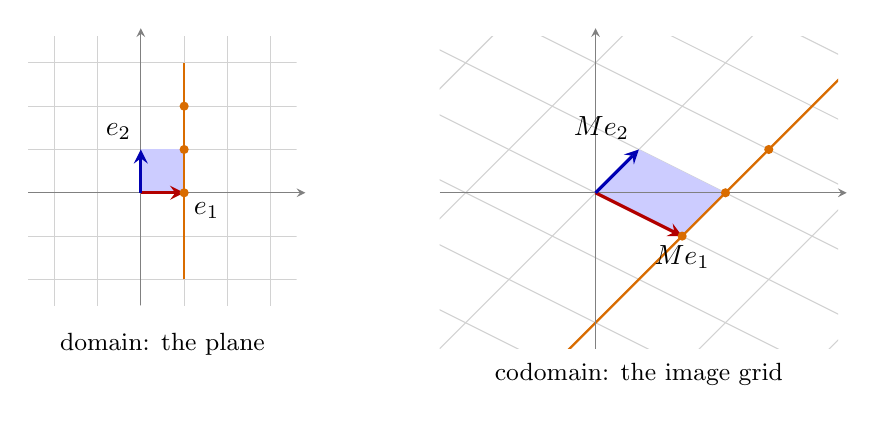
\begin{tikzpicture}[scale=0.55,>=stealth]
  \begin{scope}
    \clip (-2.6,-2.6) rectangle (3.6,3.6);
    \foreach \k in {-3,...,4}{\draw[gray!35] (\k,-3)--(\k,4); \draw[gray!35] (-3,\k)--(4,\k);}
  \end{scope}
  \draw[->,gray] (-2.6,0)--(3.8,0); \draw[->,gray] (0,-2.6)--(0,3.8);
  \fill[blue!20] (0,0) rectangle (1,1);
  \draw[thick,orange!85!black] (1,-2)--(1,3);
  \draw[->,very thick,red!70!black] (0,0)--(1,0);
  \draw[->,very thick,blue!70!black] (0,0)--(0,1);
  \foreach \t in {0,1,2}{\fill[orange!85!black] (1,\t) circle (3pt);}
  \node[below right] at (1,0) {$e_1$};
  \node[above left] at (0,1) {$e_2$};
  \node at (0.5,-3.5) {\small domain: the plane};
  \begin{scope}[xshift=10.5cm]
    \begin{scope}
      \clip (-3.6,-3.6) rectangle (5.6,3.6);
      \begin{scope}[cm={2,-1,1,1,(0,0)}]
        \foreach \k in {-6,...,6}{\draw[gray!35] (\k,-6)--(\k,6); \draw[gray!35] (-6,\k)--(6,\k);}
        \fill[blue!20] (0,0) rectangle (1,1);
        \draw[thick,orange!85!black] (1,-6)--(1,6);
      \end{scope}
    \end{scope}
    \draw[->,gray] (-3.6,0)--(5.8,0); \draw[->,gray] (0,-3.6)--(0,3.8);
    \draw[->,very thick,red!70!black] (0,0)--(2,-1);
    \draw[->,very thick,blue!70!black] (0,0)--(1,1);
    \foreach \p in {(2,-1),(3,0),(4,1)}{\fill[orange!85!black] \p circle (3pt);}
    \node[below] at (2,-1) {$Me_1$};
    \node[above left] at (1,1) {$Me_2$};
    \node at (1,-4.2) {\small codomain: the image grid};
  \end{scope}
\end{tikzpicture}
\end{center}

\textbf{Figure.} Left: the standard grid, the vectors $\bv{e}_1,\bv{e}_2$, the unit square (shaded) and three equally spaced points on the line $x_1=1$. Right: their images under $M$. The grid of squares becomes a grid of parallelograms, the unit square becomes the parallelogram with sides $M\bv{e}_1=\bv{m}_1$ and $M\bv{e}_2=\bv{m}_2$ (the columns of $M$, as in Example~\ref{1.4-ex:ei}), the origin stays put, and straight lines stay straight, with equally spaced points staying equally spaced. The next pages explain why these features are no accident.

\begin{exmp}{Three matrix transformations of the plane}{corners}
Look at what each transformation does to the corners $(0,0),(1,0),(1,1),(0,1)$ of the unit square.

\textbf{(a) A shear.} $S=\begin{bmatrix}1&1\\0&1\end{bmatrix}$, so $S(x_1,x_2)=(x_1+x_2,\ x_2)$. The corners go to $(0,0),(1,0),(2,1),(1,1)$. Each horizontal line slides to the right by an amount equal to its height; the $x_1$-axis does not move. The square becomes a slanted parallelogram with the same base and the same height.

\textbf{(b) A projection.} $P=\begin{bmatrix}1&0\\0&0\end{bmatrix}$, so $P(x_1,x_2)=(x_1,0)$. The corners go to $(0,0),(1,0),(1,0),(0,0)$. The whole plane is crushed onto the $x_1$-axis; every vertical line collapses to a single point. The range is only the $x_1$-axis, not all of $\R^2$.

\textbf{(c) A dilation.} $D=\begin{bmatrix}2&0\\0&2\end{bmatrix}$, so $D\bv{x}=2\bv{x}$. The corners go to $(0,0),(2,0),(2,2),(0,2)$: every vector is doubled and the square is enlarged, with no turning or slanting.
\end{exmp}

\begin{kc}{Image of a square}{square}
Let $A=\begin{bmatrix}1&2\\0&1\end{bmatrix}$. Find the images of the four corners of the unit square and sketch the image. Where does the diagonal from $(0,0)$ to $(1,1)$ go?
\end{kc}

% ---------------------------------------------------------------------
\subsection*{Linear transformations}

The proof of Theorem~\ref{1.4-thm:linear} used only the definition of $A\bv{x}$, and the conclusion, $A(\bv{u}+\bv{v})=A\bv{u}+A\bv{v}$ and $A(c\bv{u})=cA\bv{u}$, is exactly what the pictures above display: sums and scalar multiples are carried to sums and scalar multiples. We take these two rules as the definition of the class of transformations that matters.

\begin{defn}{Linear transformation}{linear}
A transformation $T:\R^n\to\R^m$ is \emph{linear} if
\begin{enumerate}[label=(\roman*),itemsep=1pt]
  \item $T(\bv{u}+\bv{v})=T(\bv{u})+T(\bv{v})$ for all $\bv{u},\bv{v}$ in the domain of $T$, and
  \item $T(c\bv{u})=c\,T(\bv{u})$ for all $\bv{u}$ in the domain of $T$ and all scalars $c$.
\end{enumerate}
\end{defn}

Both rules say that $T$ is \emph{compatible with the vector operations}: adding (or scaling) first and then applying $T$ gives the same result as applying $T$ first and then adding (or scaling). The definition mentions nothing about coordinates, rows or columns. That is deliberate: in Chapter~4 the ``vectors'' will be polynomials and functions, and the same two rules will define linearity there.

\begin{thm}{Matrix transformations are linear}{matlin}
Every matrix transformation $T(\bv{x})=A\bv{x}$ is a linear transformation.
\end{thm}

\begin{proof}
This is Theorem~\ref{1.4-thm:linear}.
\end{proof}

\begin{thm}{Properties of linear transformations}{props}
If $T$ is a linear transformation, then
\begin{enumerate}[label=(\alph*),itemsep=1pt]
  \item $T(\bv{0})=\bv{0}$;
  \item $T(c\bv{u}+d\bv{v})=c\,T(\bv{u})+d\,T(\bv{v})$ for all vectors $\bv{u},\bv{v}$ and all scalars $c,d$;
  \item $T(c_1\bv{v}_1+\cdots+c_p\bv{v}_p)=c_1T(\bv{v}_1)+\cdots+c_pT(\bv{v}_p)$ for all vectors $\bv{v}_j$ and scalars $c_j$ \ (the \emph{superposition principle}).
\end{enumerate}
\end{thm}

\begin{proof}
(a)~For any vector $\bv{u}$ in the domain, $\bv{0}=0\cdot\bv{u}$, so $T(\bv{0})=T(0\cdot\bv{u})=0\cdot T(\bv{u})=\bv{0}$ by rule~(ii). (b)~Rule~(i) and then rule~(ii) give $T(c\bv{u}+d\bv{v})=T(c\bv{u})+T(d\bv{v})=cT(\bv{u})+dT(\bv{v})$. (c)~Apply~(b) repeatedly (induction on $p$): $T(c_1\bv{v}_1+\cdots+c_p\bv{v}_p)=c_1T(\bv{v}_1)+T(c_2\bv{v}_2+\cdots+c_p\bv{v}_p)$, and so on.
\end{proof}

\begin{think}{A necessary test, but is it enough?}{origin}
Theorem~\ref{thm:props}(a) says every linear transformation fixes the origin. (a)~Use this to reject the formula $T(x_1,x_2)=(x_1+2,\,x_2)$ at once; what does this transformation do to the plane geometrically? (b)~Does the converse hold: if $T(\bv{0})=\bv{0}$, must $T$ be linear? Test $T(x_1,x_2)=(x_1x_2,\,x_2)$.
\end{think}

\begin{think}{Two rules or one?}{onerule}
Show that $T$ satisfies both rules of Definition~\ref{def:linear} if and only if $T(c\bv{u}+d\bv{v})=cT(\bv{u})+dT(\bv{v})$ for all $\bv{u},\bv{v},c,d$. Which choices of $c$ and $d$ turn the one-line rule back into rule~(i) and rule~(ii)? Why might a mathematician prefer one rule, and a student two?
\end{think}

\begin{exmp}{Testing four formulas}{testing}
Decide whether each transformation is linear.

\textbf{(a)} $T(x_1,x_2)=(2x_1-x_2,\ x_1+3x_2,\ 4x_2)$, from $\R^2$ to $\R^3$. Every output entry is a sum of constant multiples of $x_1$ and $x_2$, so by the row--column rule (Theorem~\ref{1.4-thm:rowcol}) $T(\bv{x})=K\bv{x}$ with $K=\begin{bmatrix}2&-1\\1&3\\0&4\end{bmatrix}$. It is a matrix transformation, hence linear (Theorem~\ref{thm:matlin}).

\textbf{(b)} $T(x_1,x_2)=(x_1+2,\ x_2)$. Here $T(\bv{0})=(2,0)\neq\bv{0}$, so $T$ is \emph{not} linear (Theorem~\ref{thm:props}(a)). Geometrically it slides the whole plane two units to the right.

\textbf{(c)} $T(x_1,x_2)=(x_1x_2,\ x_2)$. The origin passes the test, $T(\bv{0})=\bv{0}$, so we must look for a counterexample. Take $\bv{u}=(1,1)$ and $c=2$: $T(2\bv{u})=T(2,2)=(4,2)$, but $2T(\bv{u})=2(1,1)=(2,2)$. Rule~(ii) fails, so $T$ is not linear. (The product $x_1x_2$ is the culprit.)

\textbf{(d)} $T(x_1,x_2)=(|x_1|,\ x_2)$. Again $T(\bv{0})=\bv{0}$. Take $\bv{u}=(1,0)$ and $c=-1$: $T(-\bv{u})=T(-1,0)=(1,0)$, but $-T(\bv{u})=(-1,0)$. Rule~(ii) fails, so $T$ is not linear.

\emph{Moral.} One counterexample settles ``not linear''. To settle ``linear'' you need an argument for \emph{all} $\bv{u},\bv{v},c$; usually the argument is ``it is a matrix transformation''.
\end{exmp}

\begin{proc}{Is $T$ linear?}{testproc}
\begin{enumerate}
  \item Compute $T(\bv{0})$. If it is not $\bv{0}$, stop: $T$ is not linear.
  \item If every entry of $T(\bv{x})$ is a sum of constant multiples of the entries of $\bv{x}$ (no products of entries, no powers, no absolute values, no added constants), write down the matrix whose $j$th column holds the coefficients of $x_j$. Then $T(\bv{x})=A\bv{x}$ and $T$ is linear.
  \item Otherwise look for a counterexample to rule~(i) or rule~(ii) with small numbers (try $c=2$ or $c=-1$, and $\bv{u},\bv{v}$ among the vectors $\bv{e}_j$ or their sums). If you cannot find one after an honest search, prove both rules for general $\bv{u},\bv{v},c$.
\end{enumerate}
\end{proc}

\begin{kc}{Linear or not?}{linearornot}
Decide whether each transformation is linear, giving a matrix or a specific counterexample.
(a)~$T(x_1,x_2)=(x_1-x_2,\ 3x_2)$; \ (b)~$T(x_1,x_2)=(x_1,\ x_2+1)$; \ (c)~$T(x_1,x_2)=(x_1^2,\ x_2)$; \ (d)~$T(x_1,x_2,x_3)=x_1+x_2+x_3$, from $\R^3$ to $\R$; \ (e)~$T(\bv{x})=5\bv{x}$ for $\bv{x}$ in $\R^n$.
\end{kc}

\begin{center}
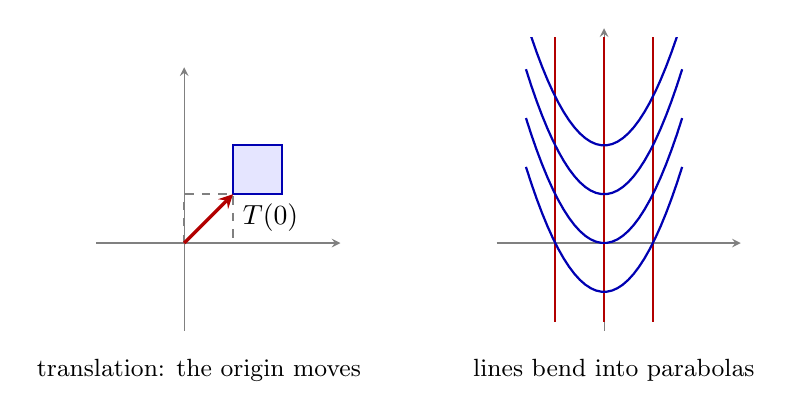
\begin{tikzpicture}[scale=0.62,>=stealth]
  \draw[->,gray] (-1.8,0)--(3.2,0); \draw[->,gray] (0,-1.8)--(0,3.6);
  \draw[gray,thick,dashed] (0,0) rectangle (1,1);
  \draw[thick,blue!70!black,fill=blue!10] (1,1) rectangle (2,2);
  \draw[->,very thick,red!70!black] (0,0)--(1,1);
  \node[below right] at (1,1) {$T(0)$};
  \node at (0.3,-2.6) {\small translation: the origin moves};
  \begin{scope}[xshift=8.6cm]
    \draw[->,gray] (-2.2,0)--(2.8,0); \draw[->,gray] (0,-1.8)--(0,4.4);
    \begin{scope}
      \clip (-2.0,-1.6) rectangle (2.4,4.2);
      \foreach \j in {-1,0,1}{\draw[thick,red!70!black] (\j,-2)--(\j,4.6);}
      \foreach \k in {-1,0,1,2}{\draw[thick,blue!70!black,domain=-1.6:1.6,samples=30] plot (\x,{\k+\x*\x});}
    \end{scope}
    \node at (0.2,-2.6) {\small lines bend into parabolas};
  \end{scope}
\end{tikzpicture}
\end{center}

\textbf{Figure.} Two transformations that are not linear. Left: the translation $T(\bv{x})=\bv{x}+(1,1)$ carries the unit square (dashed) to a copy of itself but moves the origin to $(1,1)$. Right: $T(x_1,x_2)=(x_1,\ x_2+x_1^2)$ keeps vertical lines vertical and fixes the origin, yet it bends every horizontal line into a parabola. Linear transformations do neither: they fix the origin and never bend a line.

% ---------------------------------------------------------------------
\subsection*{Lines, squares and the parallelogram rule}

Recall the parallelogram rule of Section~1.3: $\bv{u}+\bv{v}$ is the far corner of the parallelogram spanned by $\bv{u}$ and $\bv{v}$. Rule~(i) says that a linear transformation maps this far corner to the far corner of the image parallelogram.

\begin{center}
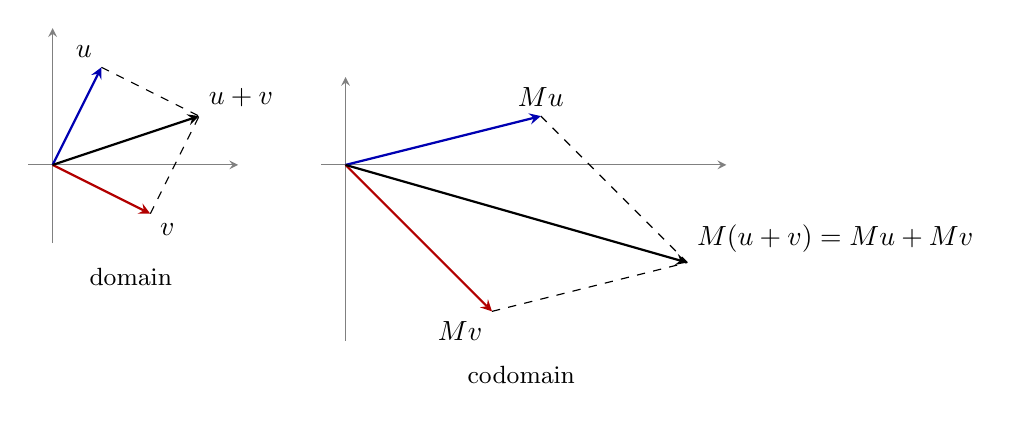
\begin{tikzpicture}[scale=0.62,>=stealth]
  \draw[->,gray] (-0.5,0)--(3.8,0); \draw[->,gray] (0,-1.6)--(0,2.8);
  \draw[dashed] (1,2)--(3,1); \draw[dashed] (2,-1)--(3,1);
  \draw[->,thick,blue!70!black] (0,0)--(1,2);
  \draw[->,thick,red!70!black] (0,0)--(2,-1);
  \draw[->,thick] (0,0)--(3,1);
  \node[above left] at (1,2) {$u$};
  \node[below right] at (2,-1) {$v$};
  \node[above right] at (3,1) {$u+v$};
  \node at (1.6,-2.3) {\small domain};
  \begin{scope}[xshift=6cm]
    \draw[->,gray] (-0.5,0)--(7.8,0); \draw[->,gray] (0,-3.6)--(0,1.8);
    \draw[dashed] (4,1)--(7,-2); \draw[dashed] (3,-3)--(7,-2);
    \draw[->,thick,blue!70!black] (0,0)--(4,1);
    \draw[->,thick,red!70!black] (0,0)--(3,-3);
    \draw[->,thick] (0,0)--(7,-2);
    \node[above] at (4,1) {$Mu$};
    \node[below left] at (3,-3) {$Mv$};
    \node[above right] at (7,-2) {$M(u+v)=Mu+Mv$};
    \node at (3.6,-4.3) {\small codomain};
  \end{scope}
\end{tikzpicture}
\end{center}

\textbf{Figure.} For $M$ as above, $\bv{u}=(1,2)$ and $\bv{v}=(2,-1)$: $M\bv{u}=(4,1)$, $M\bv{v}=(3,-3)$, and $M(\bv{u}+\bv{v})=M(3,1)=(7,-2)=M\bv{u}+M\bv{v}$.

\begin{thm}{Lines go to lines}{lines}
Let $T:\R^n\to\R^m$ be linear, and let $\bv{p}$ and $\bv{d}$ be vectors in $\R^n$. Then
\[
T(\bv{p}+t\bv{d})=T(\bv{p})+t\,T(\bv{d})\qquad\text{for every real number }t.
\]
So the image of the line through $\bv{p}$ with direction $\bv{d}$ is the line through $T(\bv{p})$ with direction $T(\bv{d})$, or the single point $T(\bv{p})$ if $T(\bv{d})=\bv{0}$. Moreover, points that are equally spaced in the parameter $t$ go to points that are equally spaced in $t$.
\end{thm}

\begin{proof}
This is Theorem~\ref{thm:props}(b) with $c=1$ and $d=t$.
\end{proof}

The same computation applied to the unit square in the plane: every point of it has the form $s\bv{e}_1+t\bv{e}_2$ with $0\le s,t\le1$, and $T(s\bv{e}_1+t\bv{e}_2)=sT(\bv{e}_1)+tT(\bv{e}_2)$. So the image of the unit square is the parallelogram spanned by $T(\bv{e}_1)$ and $T(\bv{e}_2)$, flattened to a segment or a point when these two vectors are dependent (Section~1.7).

\begin{think}{What cannot a linear map do?}{shapes}
For each claim, give a linear $T:\R^2\to\R^2$ that does it, or explain why none exists: (a)~turns a line into a curve; (b)~turns the unit square into a triangle; (c)~turns a segment into a longer segment; (d)~turns the unit square into a segment; (e)~turns a segment into a parallelogram. What do (d) and (e) say about ``flat'' objects?
\end{think}

% ---------------------------------------------------------------------
\subsection*{A linear map is determined by a few values}

By superposition, if you know $T$ on some vectors you know it on every combination of them.

\begin{exmp}{Finding $T(\bv{w})$ and a matrix from two values}{values}
Let $T:\R^2\to\R^3$ be linear with $T(\bv{u})=(2,-1,3)$ and $T(\bv{v})=(0,4,1)$, where $\bv{u}=(1,2)$ and $\bv{v}=(1,3)$. Find $T(\bv{w})$ for $\bv{w}=(3,5)$, and find $T(\bv{e}_1)$ and $T(\bv{e}_2)$.

\textbf{Solution.} We need $\bv{w}$, $\bv{e}_1$ and $\bv{e}_2$ as combinations of $\bv{u}$ and $\bv{v}$. All three weight problems have the same coefficient matrix $[\bv{u}\ \bv{v}]$, so solve them together:
\begin{align*}
\begin{amat}{cc|ccc}1&1&3&1&0\\2&3&5&0&1\end{amat}
&\rops{R_2-2R_1}
\begin{amat}{cc|ccc}1&1&3&1&0\\0&1&-1&-2&1\end{amat}
\rops{R_1-R_2}
\begin{amat}{cc|ccc}1&0&4&3&-1\\0&1&-1&-2&1\end{amat}.
\end{align*}
Reading the columns of the right side: $\bv{w}=4\bv{u}-\bv{v}$, \ $\bv{e}_1=3\bv{u}-2\bv{v}$, \ $\bv{e}_2=-\bv{u}+\bv{v}$. By superposition,
\begin{align*}
T(\bv{w})&=4T(\bv{u})-T(\bv{v})=(8,-4,12)-(0,4,1)=(8,-8,11),\\
T(\bv{e}_1)&=3T(\bv{u})-2T(\bv{v})=(6,-3,9)-(0,8,2)=(6,-11,7),\\
T(\bv{e}_2)&=-T(\bv{u})+T(\bv{v})=(-2,1,-3)+(0,4,1)=(-2,5,-2).
\end{align*}
Since $T(\bv{x})=x_1T(\bv{e}_1)+x_2T(\bv{e}_2)$, the matrix $A=\begin{bmatrix}6&-2\\-11&5\\7&-2\end{bmatrix}$ with columns $T(\bv{e}_1),T(\bv{e}_2)$ satisfies $T(\bv{x})=A\bv{x}$. Check: $A\bv{u}=(6-4,\ -11+10,\ 7-4)=(2,-1,3)$, \ $A\bv{v}=(6-6,\ -11+15,\ 7-6)=(0,4,1)$. \ $\checkmark$

\emph{Why it worked.} The vectors $\bv{u},\bv{v}$ are independent (neither is a multiple of the other), so by Theorem~\ref{1.7-thm:unique} every vector of their span, which is all of $\R^2$ here, has \emph{unique} weights. A different recipe could not have produced a different $T(\bv{w})$.
\end{exmp}

\begin{kc}{Use linearity}{superpos}
Let $T:\R^2\to\R^2$ be linear with $T(\bv{u})=(1,2)$ and $T(\bv{v})=(-3,1)$. Compute $T(2\bv{u}+\bv{v})$, $T(\bv{u}-3\bv{v})$ and $T(\bv{0})$ \emph{without} knowing $\bv{u}$ or $\bv{v}$.
\end{kc}

\begin{think}{How many values are enough?}{determined}
(a)~Let $\bv{v}=2\bv{u}$. Can a linear $T$ have $T(\bv{u})=(1,0)$ and $T(\bv{v})=(0,1)$? (b)~If $\bv{u},\bv{v}$ are independent vectors in $\R^3$ and $T(\bv{u}),T(\bv{v})$ are known, can you compute $T(\bv{w})$ for \emph{every} $\bv{w}$ in $\R^3$? (c)~How many vectors in $\R^n$ do you expect to need to know the images of?
\end{think}

% ---------------------------------------------------------------------
\subsection*{Preimages: two inputs, one output}

When do two different inputs have the same image?

\begin{thm}{Collisions}{sameimage}
Let $T$ be linear. Then $T(\bv{x})=T(\bv{y})$ if and only if $T(\bv{x}-\bv{y})=\bv{0}$.
\end{thm}

\begin{proof}
By Theorem~\ref{thm:props}(b), $T(\bv{x})-T(\bv{y})=T(\bv{x}-\bv{y})$. So the left side is $\bv{0}$ exactly when the two images agree.
\end{proof}

In words: two inputs collide exactly when their \emph{difference} is sent to $\bv{0}$. For a matrix transformation the vectors sent to $\bv{0}$ are the solutions of $A\bv{x}=\bv{0}$, so the preimage of $\bv{b}$ is a particular solution plus all solutions of $A\bv{x}=\bv{0}$: this is Theorem~\ref{1.5-thm:translate}, now with a picture.

\begin{exmp}{The preimage of a point is a line}{fibres}
Let $A=\begin{bmatrix}1&2\\2&4\end{bmatrix}$ and $T(\bv{x})=A\bv{x}$. Then $T(\bv{x})=(x_1+2x_2)\,(1,2)$: every image is a multiple of $(1,2)$. Find all $\bv{x}$ with $T(\bv{x})=(2,4)$, and decide whether $(2,3)$ is in the range.

\textbf{Solution.}
\begin{align*}
\begin{amat}{cc|c}1&2&2\\2&4&4\end{amat}
&\rops{R_2-2R_1}
\begin{amat}{cc|c}1&2&2\\0&0&0\end{amat},
\qquad
\begin{amat}{cc|c}1&2&2\\2&4&3\end{amat}
\rops{R_2-2R_1}
\begin{amat}{cc|c}1&2&2\\0&0&-1\end{amat}.
\end{align*}
The first system is consistent with $x_2$ free and $x_1=2-2x_2$:
\[
\bv{x}=\begin{bmatrix}2\\0\end{bmatrix}+x_2\begin{bmatrix}-2\\1\end{bmatrix}.
\]
So the preimage of $(2,4)$ is the line through $\bv{p}=(2,0)$ parallel to $(-2,1)$, and $(-2,1)$ spans the vectors sent to $\bv{0}$. Check: $A(2,0)=(2,4)$ and $A(-2,1)=(0,0)$. \ $\checkmark$ The second system has a row $[\,0\ \ 0\mid-1\,]$, so it is inconsistent: $(2,3)$ is not an image.

\emph{Picture.} The line $x_1+2x_2=c$ in the domain is sent to the single point $c\,(1,2)$. The whole plane is folded onto the line $\Span\{(1,2)\}$, and each point of that line has an entire line of preimages (below, $c=0$ and $c=2$).
\end{exmp}

\begin{center}
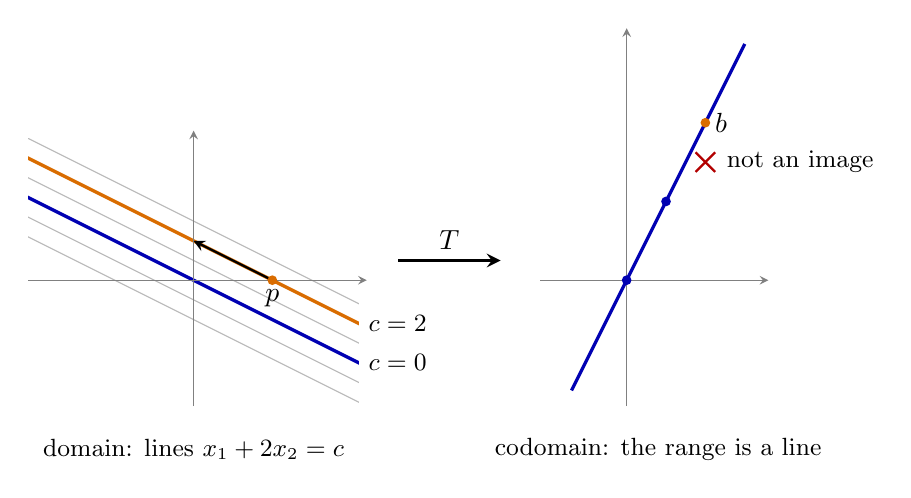
\begin{tikzpicture}[scale=0.5,>=stealth]
  \begin{scope}
    \clip (-4.2,-3.2) rectangle (4.2,3.6);
    \foreach \c in {-2,-1,1,3}{\draw[gray!55] (-5,{(\c+5)/2}) -- (5,{(\c-5)/2});}
    \draw[very thick,blue!70!black] (-5,2.5)--(5,-2.5);
    \draw[very thick,orange!85!black] (-5,3.5)--(5,-1.5);
  \end{scope}
  \draw[->,gray] (-4.2,0)--(4.4,0); \draw[->,gray] (0,-3.2)--(0,3.8);
  \draw[->,thick,black] (2,0)--(0,1);
  \fill[orange!85!black] (2,0) circle (3.5pt);
  \node[below] at (2,0) {$p$};
  \node[right] at (4.2,-2.1) {\small $c=0$};
  \node[right] at (4.2,-1.1) {\small $c=2$};
  \node at (0,-4.3) {\small domain: lines $x_1+2x_2=c$};
  \draw[->,very thick] (5.2,0.5)--(7.8,0.5) node[midway,above] {$T$};
  \begin{scope}[xshift=11cm]
    \draw[->,gray] (-2.2,0)--(3.6,0); \draw[->,gray] (0,-3.2)--(0,6.4);
    \draw[very thick,blue!70!black] (-1.4,-2.8)--(3,6);
    \fill[blue!70!black] (0,0) circle (3.5pt);
    \fill[blue!70!black] (1,2) circle (3.5pt);
    \fill[orange!85!black] (2,4) circle (3.5pt);
    \draw[thick,red!70!black] (1.75,2.75)--(2.25,3.25) (1.75,3.25)--(2.25,2.75);
    \node[right] at (2,4) {$b$};
    \node[right] at (2.3,3) {\small not an image};
    \node at (0.8,-4.3) {\small codomain: the range is a line};
  \end{scope}
\end{tikzpicture}
\end{center}

\textbf{Figure.} Each line $x_1+2x_2=c$ (left) is crushed to the point $c\,(1,2)$ (right). The blue line $c=0$ is the set of vectors sent to $\bv{0}$; the orange line $c=2$ is the preimage of $\bv{b}=(2,4)$. The cross marks a point of the codomain, $(2,3)$, that no input reaches.

\begin{think}{Same output, different inputs}{fibres}
(a)~In Example~\ref{ex:fibres}, how many inputs share the output $(2,4)$? Which inputs are sent to $\bv{0}$? (b)~Suppose a linear $T$ sends two different vectors $\bv{x}\ne\bv{y}$ to the same image. Why must there be infinitely many inputs with that image? (c)~At the end of Section~1.7 you were asked: if the columns of $A$ are independent, can two different inputs have the same output? Answer it using Theorem~\ref{thm:sameimage}.
\end{think}

% ---------------------------------------------------------------------
\subsection*{Linear maps and independence}

Section~1.7 asked when a combination of vectors can give $\bv{0}$. A linear transformation carries such a combination along.

\begin{thm}{Linear maps and dependence}{depimages}
Let $T:\R^n\to\R^m$ be linear and let $\bv{v}_1,\dots,\bv{v}_p$ be vectors in $\R^n$.
\begin{enumerate}[label=(\alph*),itemsep=1pt]
  \item If $\{\bv{v}_1,\dots,\bv{v}_p\}$ is dependent, then $\{T(\bv{v}_1),\dots,T(\bv{v}_p)\}$ is dependent. Equivalently, if the images are independent, then so are the $\bv{v}_j$.
  \item If $T(\bv{x})=A\bv{x}$ and the columns of $A$ are independent, then independent $\bv{v}_1,\dots,\bv{v}_p$ have independent images.
\end{enumerate}
\end{thm}

\begin{proof}
(a)~Take a dependence relation $c_1\bv{v}_1+\cdots+c_p\bv{v}_p=\bv{0}$ with not all $c_j=0$. Apply $T$ and use Theorem~\ref{thm:props}: $c_1T(\bv{v}_1)+\cdots+c_pT(\bv{v}_p)=T(\bv{0})=\bv{0}$. This is a dependence relation among the images, with the \emph{same} weights.

(b)~Suppose $c_1T(\bv{v}_1)+\cdots+c_pT(\bv{v}_p)=\bv{0}$. Then $A(c_1\bv{v}_1+\cdots+c_p\bv{v}_p)=\bv{0}$. Since the columns of $A$ are independent, $A\bv{x}=\bv{0}$ has only the trivial solution (Theorem~\ref{1.7-thm:cols}), so $c_1\bv{v}_1+\cdots+c_p\bv{v}_p=\bv{0}$. As the $\bv{v}_j$ are independent, every $c_j=0$.
\end{proof}

\begin{exmp}{Independence kept, independence lost}{indimg}
Let $A=\begin{bmatrix}1&2\\0&1\\1&1\end{bmatrix}$ and $B=\begin{bmatrix}1&2\\2&4\end{bmatrix}$. Row reducing $[A\ \bv{0}]$ and $[B\ \bv{0}]$:
\begin{align*}
\begin{amat}{cc|c}1&2&0\\0&1&0\\1&1&0\end{amat}
&\rops{R_3-R_1}
\begin{amat}{cc|c}1&2&0\\0&1&0\\0&-1&0\end{amat}
\rops{R_3+R_2}
\begin{amat}{cc|c}1&2&0\\0&1&0\\0&0&0\end{amat},
\qquad
\begin{amat}{cc|c}1&2&0\\2&4&0\end{amat}
\rops{R_2-2R_1}
\begin{amat}{cc|c}1&2&0\\0&0&0\end{amat}.
\end{align*}
The columns of $A$ are independent (two pivots); the columns of $B$ are dependent (column $2$ is free; indeed $2\bv{b}_1-\bv{b}_2=\bv{0}$). Take the independent vectors $\bv{v}_1=(1,1)$ and $\bv{v}_2=(1,-1)$.

For $A$: $A\bv{v}_1=(3,1,2)$ and $A\bv{v}_2=(-1,-1,0)$. Neither is a multiple of the other, so the images are independent, as Theorem~\ref{thm:depimages}(b) promises.

For $B$: the independent vectors $\bv{e}_1,\bv{e}_2$ have images $B\bv{e}_1=(1,2)$ and $B\bv{e}_2=(2,4)=2(1,2)$, which are dependent. Independence was \emph{lost}, and Theorem~\ref{thm:depimages}(b) does not apply because the columns of $B$ are dependent.
\end{exmp}

\begin{kc}{Does independence survive?}{images2}
(a)~For $T(x_1,x_2)=(x_1,\ x_2,\ x_1+x_2)$, are $T(\bv{e}_1)$ and $T(\bv{e}_2)$ independent? (b)~For the projection $P(x_1,x_2)=(x_1,0)$, are $P(\bv{e}_1)$ and $P(\bv{e}_2)$ independent? (c)~Which of the two maps sends a nonzero vector to $\bv{0}$?
\end{kc}

\begin{think}{Is the converse true?}{converse}
If $T(\bv{v}_1),T(\bv{v}_2)$ are dependent, must $\bv{v}_1,\bv{v}_2$ be dependent? Find a linear $T$ and vectors showing the answer is no. Then use Theorem~\ref{thm:depimages}(b) to find a property of $T$ that makes the converse true.
\end{think}

% ---------------------------------------------------------------------
\subsection*{Linear transformations without a matrix in sight}

The definition of linearity never mentions matrices, so it applies to any objects that can be added and scaled. Polynomials are the first example; we record $a+bt+ct^2$ by its coefficient vector $(a,b,c)$ in $\R^3$, as in Section~1.7.

\begin{exmp}{Differentiation and evaluation}{poly}
Define $D$ and $E$ on polynomials of degree at most $2$ by $D(p)=p'$ and $E(p)=p(2)$. For $p(t)=a+bt+ct^2$ we have $D(p)=b+2ct$ and $E(p)=a+2b+4c$. In coefficient vectors,
\[
D:\ (a,b,c)\mapsto(b,\ 2c),\qquad E:\ (a,b,c)\mapsto a+2b+4c,
\]
so $D$ is the matrix transformation $\bv{x}\mapsto\begin{bmatrix}0&1&0\\0&0&2\end{bmatrix}\bv{x}$ from $\R^3$ to $\R^2$, and $E$ is $\bv{x}\mapsto\begin{bmatrix}1&2&4\end{bmatrix}\bv{x}$ from $\R^3$ to $\R$. Both are linear. For $p(t)=3-2t+5t^2$, i.e.\ $\bv{x}=(3,-2,5)$: $p'(t)=-2+10t$, matching $D\bv{x}=(-2,10)$; and $p(2)=3-4+20=19$, matching $E\bv{x}=3-4+20=19$.

The same linearity can be seen \emph{without} coordinates, from the rules of calculus: $(p+q)'=p'+q'$ and $(cp)'=cp'$; and $(p+q)(2)=p(2)+q(2)$ and $(cp)(2)=c\,p(2)$. By contrast $S(p)=p(2)^2$ is not linear: for the constant polynomial $p=1$ we get $S(2p)=S(2)=4$ but $2S(p)=2$.
\end{exmp}

\begin{think}{Is calculus linear?}{calc}
You know the rules $(f+g)'=f'+g'$ and $(cf)'=cf'$. In what sense is it correct to say that ``differentiation is a linear transformation''? Test the same question for (a)~$f\mapsto\int_0^1 f(t)\,dt$, (b)~$f\mapsto f(t)^2$ (squaring the function), (c)~$f\mapsto f(0)+1$.
\end{think}

\begin{exmp}{Production plans and fixed costs}{workshop}
In the workshop of Example~\ref{1.4-ex:machine} the matrix $A=\begin{bmatrix}3&1&2\\2&1&1\end{bmatrix}$ turns a production plan $\bv{x}$ (tables, chairs, stools) into resources (wood, labor): $T(\bv{x})=A\bv{x}$. For the plans $\bv{x}=(4,10,6)$ and $\bv{y}=(2,0,5)$,
\[
T(\bv{x})=(34,24),\qquad T(\bv{y})=(16,9),\qquad T(\bv{x}+\bv{y})=T(6,10,11)=(50,33)=T(\bv{x})+T(\bv{y}),
\]
and $T(3\bv{x})=(102,72)=3T(\bv{x})$. Linearity is the statement that there are no economies and no penalties of scale: the resources for two plans together are the sum of the resources, and a plan three times as large costs three times as much.

Now suppose each day starts with a fixed set-up that wastes $10$ units of wood, whatever is built. The total requirement is $N(\bv{x})=A\bv{x}+(10,0)$. Then $N(\bv{0})=(10,0)\neq\bv{0}$: even an idle workshop consumes wood, so $N$ is \emph{not} linear (Theorem~\ref{thm:props}(a)). It is a linear map followed by a shift: an \emph{affine} map.
\end{exmp}

\begin{think}{Linear, or only affine?}{affine}
The conversion from degrees Celsius to degrees Fahrenheit is $F=1.8\,C+32$. Is $C\mapsto F$ a linear transformation from $\R$ to $\R$? Check it with $C=20$ and $C=40$. Now consider the conversion of a temperature \emph{difference}: if the temperature rises by $h$ degrees Celsius, by how many degrees Fahrenheit does it rise? Is that map linear? What happened to the $32$?
\end{think}

\subsection*{Summary}
\begin{itemize}
  \item A \textbf{transformation} $T:\R^n\to\R^m$ assigns to each $\bv{x}$ in the \textbf{domain} $\R^n$ an \textbf{image} $T(\bv{x})$ in the \textbf{codomain} $\R^m$; the \textbf{range} is the set of images. The range can be smaller than the codomain.
  \item A \textbf{matrix transformation} is $T(\bv{x})=A\bv{x}$. Its range is the span of the columns of $A$; asking whether $\bv{b}$ is in the range, or what its preimages are, is asking about $A\bv{x}=\bv{b}$.
  \item $T$ is \textbf{linear} if $T(\bv{u}+\bv{v})=T(\bv{u})+T(\bv{v})$ and $T(c\bv{u})=cT(\bv{u})$. Matrix transformations are linear. Linear maps satisfy $T(\bv{0})=\bv{0}$ and \textbf{superposition}: $T(\sum c_j\bv{v}_j)=\sum c_jT(\bv{v}_j)$.
  \item To test a formula: check $T(\bv{0})=\bv{0}$; if all entries are sums of multiples of the variables it is a matrix transformation; otherwise hunt for a counterexample. One counterexample settles ``not linear''.
  \item \textbf{Geometry:} a linear map fixes the origin, sends lines to lines (or points) with equal spacing kept, and sends the unit square to the parallelogram spanned by $T(\bv{e}_1)$ and $T(\bv{e}_2)$. Nothing is bent. Translation and squaring are not linear.
  \item $T(\bv{x})=T(\bv{y})$ iff $T(\bv{x}-\bv{y})=\bv{0}$; the preimage of $\bv{b}$ is a particular solution plus the solutions of $A\bv{x}=\bv{0}$.
  \item Linear maps turn \textbf{dependence relations} into dependence relations; independence survives when only $\bv{0}$ is sent to $\bv{0}$.
  \item Polynomials, derivatives and evaluation are linear in exactly the same sense; $\bv{x}\mapsto A\bv{x}+\bv{b}$ with $\bv{b}\neq\bv{0}$ is \textbf{affine}, not linear.
\end{itemize}

\subsection*{Questions to think about before the next section}
\begin{enumerate}
  \item The rotation of the plane by $90^\circ$ counterclockwise is linear. What must $T(\bv{e}_1)$ and $T(\bv{e}_2)$ be? Guess its matrix and test it on the vector $(1,1)$.
  \item If $T:\R^2\to\R^2$ is linear and you know $T(\bv{e}_1)$ and $T(\bv{e}_2)$, do you know $T(\bv{x})$ for every $\bv{x}$? Write the formula.
  \item Which pivot condition (a pivot in every row, or in every column) decides whether every vector of the codomain is an image? Which one decides that no two inputs share an image?
\end{enumerate}

% =====================================================================
\subsection*{Example bank}

The examples below are extra practice with the problem types of this section. They use only ideas available so far, and nothing later in the course depends on them.

\begin{remark}[What's in this bank]
\begin{itemize}
  \item \textbf{Follow a figure through a matrix.} Find the image of a triangle and use it to check that lines, midpoints and independence behave as the theory says.
  \item \textbf{Decide linearity.} Test a map given in words, find the rule that breaks for a map that looks harmless, and find the values of a parameter that make a family of maps linear.
  \item \textbf{Prescribed values.} Decide whether a linear map with prescribed values at several vectors exists, and find its matrix.
\end{itemize}
\end{remark}

\subsection*{Bank: follow a figure through a matrix}

\begin{exmp}{Image of a triangle}{bankTriangle}
Let $A=\begin{bmatrix}1&2\\-1&1\end{bmatrix}$ and $T(\bv{x})=A\bv{x}$. The triangle has vertices $P=(1,1)$, $Q=(3,1)$ and $R=(1,3)$. (a)~Find the image of the triangle. (b)~Check that the midpoint of $QR$ goes to the midpoint of the image of $QR$. (c)~Explain why the image is a genuine triangle and not a segment.

\textbf{Solution.} (a)~A side of the triangle is a piece of a line, and a linear map sends a line to a line (Theorem~\ref{thm:lines}). A segment is determined by its two endpoints, so the image of each side is the segment joining the images of its endpoints. It is therefore enough to compute the images of the three vertices:
\[
\begin{bmatrix}1&2\\-1&1\end{bmatrix}\begin{bmatrix}1\\1\end{bmatrix}=\begin{bmatrix}3\\0\end{bmatrix},\qquad
\begin{bmatrix}1&2\\-1&1\end{bmatrix}\begin{bmatrix}3\\1\end{bmatrix}=\begin{bmatrix}5\\-2\end{bmatrix},\qquad
\begin{bmatrix}1&2\\-1&1\end{bmatrix}\begin{bmatrix}1\\3\end{bmatrix}=\begin{bmatrix}7\\2\end{bmatrix}.
\]
The image is the triangle with vertices $T(P)=(3,0)$, $T(Q)=(5,-2)$ and $T(R)=(7,2)$. The points inside the triangle are also carried inside: a point of the triangle is a weighted average $\bv{x}=\lambda_1P+\lambda_2Q+\lambda_3R$ with weights $\lambda_j\ge0$ adding up to $1$, and superposition gives $T(\bv{x})=\lambda_1T(P)+\lambda_2T(Q)+\lambda_3T(R)$, a weighted average of the image vertices with the \emph{same} weights.

(b)~The midpoint of $QR$ is $\tfrac12(3,1)+\tfrac12(1,3)=(2,2)$. Then
\[
\begin{bmatrix}1&2\\-1&1\end{bmatrix}\begin{bmatrix}2\\2\end{bmatrix}=\begin{bmatrix}6\\0\end{bmatrix},
\]
and the midpoint of $T(Q)=(5,-2)$ and $T(R)=(7,2)$ is $\bigl(\tfrac{5+7}{2},\tfrac{-2+2}{2}\bigr)=(6,0)$. They agree, as equal spacing along a line (Theorem~\ref{thm:lines}) says they must.

(c)~Two sides leaving $P$ are $Q-P=(2,0)$ and $R-P=(0,2)$, which are independent. The columns of $A$ are $(1,-1)$ and $(2,1)$, neither a multiple of the other, so they are independent, and by Theorem~\ref{thm:depimages}(b) the images $A(2,0)=(2,-2)$ and $A(0,2)=(4,2)$ are independent too. Two independent sides mean the image has a corner with a genuine angle, so it is a triangle with positive area. A matrix with dependent columns, such as $\begin{bmatrix}1&2\\2&4\end{bmatrix}$, would have flattened the triangle onto a segment.
\end{exmp}

\subsection*{Bank: decide linearity}

\begin{exmp}{Averaging the entries}{bankAverage}
Let $T:\R^3\to\R^3$ replace every entry of a vector by the average of the three entries:
\[
T(x_1,x_2,x_3)=\tfrac13(x_1+x_2+x_3)\,(1,1,1).
\]
(a)~Show that $T$ is linear and find its matrix. (b)~Describe the range. (c)~Find every $\bv{x}$ with $T(\bv{x})=(2,2,2)$.

\textbf{Solution.} (a)~Each entry of $T(\bv{x})$ is $\tfrac13x_1+\tfrac13x_2+\tfrac13x_3$: a sum of constant multiples of the $x_j$ and nothing else. By the row--column rule (Procedure~\ref{proc:testproc}, step~2) $T$ is the matrix transformation of
\[
K=\tfrac13\begin{bmatrix}1&1&1\\1&1&1\\1&1&1\end{bmatrix},
\]
so it is linear (Theorem~\ref{thm:matlin}).

(b)~Every image is a multiple of $(1,1,1)$, and every multiple $s(1,1,1)$ occurs: take $\bv{x}=(s,s,s)$, whose average is $s$. So the range is the line $\Span\{(1,1,1)\}$, a very small part of the codomain $\R^3$.

(c)~Multiplying the equation $K\bv{x}=(2,2,2)$ by $3$ keeps it equivalent, and then all three rows are the same equation:
\begin{align*}
\begin{amat}{ccc|c}1&1&1&6\\1&1&1&6\\1&1&1&6\end{amat}
&\rops{R_2-R_1,\ R_3-R_1}
\begin{amat}{ccc|c}1&1&1&6\\0&0&0&0\\0&0&0&0\end{amat}.
\end{align*}
The solutions form the plane $x_1+x_2+x_3=6$ (``three numbers with average $2$''), with $x_2$ and $x_3$ free. For instance $(1,2,3)$ and $(6,0,0)$ are both preimages. Their difference $(5,-2,-3)$ has entries adding up to $0$, so it is sent to $\bv{0}$, in agreement with Theorem~\ref{thm:sameimage}. The vectors sent to $\bv{0}$ are those with average $0$, the plane $x_1+x_2+x_3=0$, which is the solution set of $K\bv{x}=\bv{0}$; every preimage of $(2,2,2)$ is a translate of it (Theorem~\ref{1.5-thm:translate}).
\end{exmp}

\begin{exmp}{Sorting the entries}{bankSort}
Let $T:\R^2\to\R^2$ put the larger entry first: $T(x_1,x_2)=(\max\{x_1,x_2\},\ \min\{x_1,x_2\})$. Is $T$ linear?

\textbf{Solution.} First the quick test: $T(0,0)=(0,0)$, so $T(\bv{0})=\bv{0}$ and the origin test cannot reject $T$. The formula is not a sum of constant multiples of $x_1$ and $x_2$, so we must hunt for a counterexample. Try the two rules with small numbers.

\emph{Rule~(ii) with $c=2$.} For $\bv{u}=(3,1)$ we get $T(2\bv{u})=T(6,2)=(6,2)=2T(\bv{u})$. This works. In fact for every $c\ge0$ sorting commutes with scaling, so a search that tries only positive $c$ would never find a failure. That is why Procedure~\ref{proc:testproc} also suggests $c=-1$.

\emph{Rule~(ii) with $c=-1$.} For $\bv{u}=(1,0)$: $T(\bv{u})=(1,0)$ but $T(-\bv{u})=T(-1,0)=(0,-1)$, while $-T(\bv{u})=(-1,0)$. They differ, so rule~(ii) fails.

\emph{Rule~(i)} fails as well, with the unit vectors: $T(\bv{e}_1)=(1,0)$ and $T(\bv{e}_2)=(1,0)$, so $T(\bv{e}_1)+T(\bv{e}_2)=(2,0)$, but $T(\bv{e}_1+\bv{e}_2)=T(1,1)=(1,1)$.

One failure is enough: $T$ is \emph{not} linear. Geometrically, sorting folds the plane over along the line $x_2=x_1$. A fold bends lines: the line $x_1+x_2=1$ has the points $(1-t,t)$, and sorting sends both $(1-t,t)$ and $(t,1-t)$ to the same point, so the whole line is folded onto a single ray starting at $(\tfrac12,\tfrac12)$. Theorem~\ref{thm:lines} says a linear map would send the line to a line (or a point), so $T$ cannot be linear.
\end{exmp}

\begin{exmp}{A parameter in a map on polynomials}{bankPoly}
Polynomials $p(t)=a+bt+ct^2$ of degree at most $2$ are recorded by their coefficient vectors $(a,b,c)$ in $\R^3$. For a real number $k$ define two maps from these polynomials to $\R^2$:
\[
S_k(p)=\bigl(p(1)+k,\ p'(0)\bigr),\qquad U_k(p)=\bigl(p(1)+k\,p(0),\ p'(0)\bigr).
\]
(a)~For which $k$ is $S_k$ linear? For which $k$ is $U_k$ linear? (b)~Take $k=1$ in $U_k$ and find every polynomial with $U_1(p)=(4,2)$.

\textbf{Solution.} (a)~In coefficients, $p(1)=a+b+c$, $p(0)=a$ and $p'(0)=b$. For $S_k$ the zero polynomial goes to $S_k(0)=(k,0)$. A linear map must send $\bv{0}$ to $\bv{0}$ (Theorem~\ref{thm:props}(a)), so $S_k$ can be linear only if $k=0$; and for $k=0$ it is $(a,b,c)\mapsto(a+b+c,\ b)$, a matrix transformation, hence linear. So $S_k$ is linear exactly for $k=0$, and for every other $k$ it is affine (a linear map plus the constant shift $(k,0)$, as in Example~\ref{ex:workshop}).

For $U_k$ the constant $k$ is not added on its own; it multiplies $p(0)$. Then $U_k(p)=\bigl((1+k)a+b+c,\ b\bigr)$, and each entry is a sum of constant multiples of $a,b,c$. So $U_k$ is the matrix transformation
\[
\bv{x}\mapsto\begin{bmatrix}1+k&1&1\\0&1&0\end{bmatrix}\bv{x},
\]
and it is linear for \emph{every} $k$. The moral: the parameter does not decide linearity; what decides it is whether it appears as a coefficient (linear) or as an added constant (affine).

(b)~With $k=1$ the matrix is $\begin{bmatrix}2&1&1\\0&1&0\end{bmatrix}$. Solve $U_1(p)=(4,2)$:
\begin{align*}
\begin{amat}{ccc|c}2&1&1&4\\0&1&0&2\end{amat}
&\rops{R_1-R_2}
\begin{amat}{ccc|c}2&0&1&2\\0&1&0&2\end{amat}
\rops{\tfrac12R_1}
\begin{amat}{ccc|c}1&0&\tfrac12&1\\0&1&0&2\end{amat}.
\end{align*}
Column $3$ is free, so $c$ is free, $b=2$ and $a=1-\tfrac12c$. Every preimage has the form $p(t)=\bigl(1-\tfrac12c\bigr)+2t+ct^2$ for a real number $c$. Check with $c=2$: $p(t)=2t^2+2t$, so $p(1)+p(0)=4+0=4$ and $p'(0)=2$. \ $\checkmark$ The preimages form a line in coefficient space, parallel to $(-\tfrac12,0,1)$, the polynomial $-\tfrac12+t^2$ that $U_1$ sends to $\bv{0}$.
\end{exmp}

\subsection*{Bank: prescribed values}

\begin{exmp}{Can these values come from a linear map?}{bankValues}
Let $\bv{u}=(1,1)$, $\bv{v}=(1,-1)$ and $\bv{w}=(3,1)$ in $\R^2$. (a)~Is there a linear $T:\R^2\to\R^3$ with $T(\bv{u})=(2,1,0)$, $T(\bv{v})=(0,1,2)$ and $T(\bv{w})=(4,3,2)$? If so, find its matrix. (b)~Is there one with $T(\bv{w})=(4,3,1)$ instead, the other two values unchanged?

\textbf{Solution.} A linear map must respect every relation among its inputs, so first find the relations. Write $\bv{w}$, $\bv{e}_1$ and $\bv{e}_2$ in terms of $\bv{u}$ and $\bv{v}$; all three weight problems share the coefficient matrix $[\bv{u}\ \bv{v}]$, so we solve them together:
\begin{align*}
\begin{amat}{cc|ccc}1&1&3&1&0\\1&-1&1&0&1\end{amat}
&\rops{R_2-R_1}
\begin{amat}{cc|ccc}1&1&3&1&0\\0&-2&-2&-1&1\end{amat}\\
&\rops{-\tfrac12R_2}
\begin{amat}{cc|ccc}1&1&3&1&0\\0&1&1&\tfrac12&-\tfrac12\end{amat}\\
&\rops{R_1-R_2}
\begin{amat}{cc|ccc}1&0&2&\tfrac12&\tfrac12\\0&1&1&\tfrac12&-\tfrac12\end{amat}.
\end{align*}
Reading the columns of the right side: $\bv{w}=2\bv{u}+\bv{v}$, \ $\bv{e}_1=\tfrac12\bv{u}+\tfrac12\bv{v}$, \ $\bv{e}_2=\tfrac12\bv{u}-\tfrac12\bv{v}$.

(a)~Superposition forces $T(\bv{w})=2T(\bv{u})+T(\bv{v})=(4,2,0)+(0,1,2)=(4,3,2)$. This is the prescribed value, so the data are consistent. Because $\bv{u},\bv{v}$ span $\R^2$, they determine $T$ completely:
\[
T(\bv{e}_1)=\tfrac12(2,1,0)+\tfrac12(0,1,2)=(1,1,1),\qquad T(\bv{e}_2)=\tfrac12(2,1,0)-\tfrac12(0,1,2)=(1,0,-1),
\]
so the map exists, is unique, and has the matrix $A=\begin{bmatrix}1&1\\1&0\\1&-1\end{bmatrix}$. Check all three values: $A\bv{u}=(2,1,0)$, $A\bv{v}=(0,1,2)$, $A\bv{w}=(4,3,2)$. \ $\checkmark$

(b)~The relation $\bv{w}=2\bv{u}+\bv{v}$ still holds, so any linear $T$ would have to give $T(\bv{w})=(4,3,2)$. The requested value $(4,3,1)$ contradicts it. No such linear map exists, even though each value looks harmless on its own. This is Theorem~\ref{thm:depimages}(a) in action: the inputs $\bv{u},\bv{v},\bv{w}$ are dependent, and the outputs must be dependent with the same weights.
\end{exmp}

\subsection*{Answers and discussion}
\begin{description}[leftmargin=0pt,itemsep=5pt]
  \item[Knowledge Check \ref{kc:images}.] (a)~$A$ is $2\times3$, so the domain is $\R^3$ and the codomain is $\R^2$. (b)~By columns: $2(1,3)+1(0,-1)-1(2,0)=(2-2,\ 6-1)=(0,5)$. By rows: $1\cdot2+0\cdot1+2\cdot(-1)=0$ and $3\cdot2+(-1)\cdot1+0\cdot(-1)=5$. (c)~$\bv{x}=(2,7,0)$ works: $2+0=2$ and $6-7=-1$. It is not the only one: $(0,1,1)$ also works ($0+2=2$, \ $0-1=-1$). The third column is not a pivot column, so $x_3$ is free and there are infinitely many preimages. (d)~Yes. Row reducing gives $\begin{bmatrix}1&0&2\\0&1&6\end{bmatrix}$, with a pivot in each of the $2$ rows, so by Theorem~\ref{1.4-thm:existence} every vector of $\R^2$ is an image.
  \item[Knowledge Check \ref{kc:square}.] The corners $(0,0),(1,0),(1,1),(0,1)$ go to $(0,0),\ (1,0),\ (1+2,\ 1)=(3,1),\ (2,1)$: a slanted parallelogram with vertices $(0,0),(1,0),(3,1),(2,1)$, spanned by the columns $(1,0)$ and $(2,1)$. The diagonal from $(0,0)$ to $(1,1)$ goes to the segment from $(0,0)$ to $(3,1)$ (the image of a segment is a segment, and its endpoints go to the images of its endpoints).
  \item[Knowledge Check \ref{kc:linearornot}.] (a)~Linear: $T(\bv{x})=\begin{bmatrix}1&-1\\0&3\end{bmatrix}\bv{x}$. (b)~Not linear: $T(\bv{0})=(0,1)\neq\bv{0}$. (c)~Not linear: $T(2\bv{e}_1)=T(2,0)=(4,0)$, but $2T(\bv{e}_1)=2(1,0)=(2,0)$. (d)~Linear: $T(\bv{x})=\begin{bmatrix}1&1&1\end{bmatrix}\bv{x}$, a $1\times3$ matrix. (e)~Linear: $T(\bv{x})=5I\bv{x}$; directly, $5(\bv{x}+\bv{y})=5\bv{x}+5\bv{y}$ and $5(c\bv{x})=c(5\bv{x})$.
  \item[Knowledge Check \ref{kc:superpos}.] $T(2\bv{u}+\bv{v})=2(1,2)+(-3,1)=(-1,5)$. \ $T(\bv{u}-3\bv{v})=(1,2)-3(-3,1)=(10,-1)$. \ $T(\bv{0})=\bv{0}$ by Theorem~\ref{thm:props}(a). Superposition lets us find $T$ of any combination of $\bv{u}$ and $\bv{v}$; it says nothing about $T(\bv{z})$ for a $\bv{z}$ that is not such a combination.
  \item[Knowledge Check \ref{kc:images2}.] (a)~$T(\bv{e}_1)=(1,0,1)$ and $T(\bv{e}_2)=(0,1,1)$ are independent (neither is a multiple of the other). (b)~$P(\bv{e}_1)=(1,0)$ and $P(\bv{e}_2)=(0,0)=\bv{0}$: a set containing $\bv{0}$ is dependent, so independence was lost although $\bv{e}_1,\bv{e}_2$ are independent. (c)~$P$ sends the nonzero vector $\bv{e}_2$ to $\bv{0}$. The first map sends only $\bv{0}$ to $\bv{0}$ (its columns $(1,0,1),(0,1,1)$ are independent), and it keeps independence, as in Theorem~\ref{thm:depimages}(b).
  \item[Pause and think \ref{think:origin}.] (a)~Here $T(\bv{0})=(2,0)\neq\bv{0}$, so $T$ cannot be linear. Geometrically $T$ is a translation: every vector slides two units to the right, so the origin moves. (b)~No. For $T(x_1,x_2)=(x_1x_2,x_2)$ we have $T(\bv{0})=\bv{0}$, but $T(1,1)=(1,1)$ and $T(2,2)=(4,2)\neq2T(1,1)=(2,2)$. So $T(\bv{0})=\bv{0}$ is a quick \emph{necessary} test that can reject a formula but can never prove linearity.
  \item[Pause and think \ref{think:onerule}.] If both rules hold, $T(c\bv{u}+d\bv{v})=T(c\bv{u})+T(d\bv{v})=cT(\bv{u})+dT(\bv{v})$. Conversely, the one-line rule with $c=d=1$ is rule~(i), and with $d=0$ it is $T(c\bv{u})=cT(\bv{u})+0\cdot T(\bv{v})=cT(\bv{u})$, which is rule~(ii). One rule is a single statement to cite and to use (it carries a whole linear combination at once). Two rules separate ``adding'' from ``scaling'', so a failure is easier to diagnose and a counterexample easier to find. Either way: $T$ respects the only two operations vectors have.
  \item[Pause and think \ref{think:shapes}.] (a)~Impossible: by Theorem~\ref{thm:lines} the image of a line is a line or a point. (b)~Impossible: the image of the unit square is $\{sT(\bv{e}_1)+tT(\bv{e}_2)\}$, a parallelogram, or a segment or a point if $T(\bv{e}_1),T(\bv{e}_2)$ are dependent. A triangle has the wrong shape. (c)~Possible: the dilation $T(\bv{x})=3\bv{x}$ triples every length. (d)~Possible: the projection $P(x_1,x_2)=(x_1,0)$ sends the square to the segment from $(0,0)$ to $(1,0)$. (e)~Impossible: the image of a segment is a segment or a point. So a linear map can flatten (a parallelogram to a segment, a segment to a point), but it can never create dimension: flat things stay flat or get flatter.
  \item[Pause and think \ref{think:determined}.] (a)~No. If $\bv{v}=2\bv{u}$ then $T(\bv{v})=T(2\bv{u})=2T(\bv{u})=(2,0)\neq(0,1)$. A dependence relation among the inputs ($\bv{v}-2\bv{u}=\bv{0}$) forces the same relation among the images, so the prescribed values must respect it (Theorem~\ref{thm:depimages}(a)). (b)~Only for $\bv{w}$ in $\Span\{\bv{u},\bv{v}\}$, a plane. For a $\bv{w}$ outside it, the values on $\bv{u}$ and $\bv{v}$ say nothing about $T(\bv{w})$. (c)~Enough vectors that every vector of $\R^n$ is a combination of them with known weights: Section~1.9 will show that the $n$ vectors $\bv{e}_1,\dots,\bv{e}_n$ suffice.
  \item[Pause and think \ref{think:fibres}.] (a)~Infinitely many: the whole line $(2,0)+t(-2,1)$. The inputs sent to $\bv{0}$ are the multiples of $(-2,1)$. (b)~Put $\bv{d}=\bv{y}-\bv{x}\neq\bv{0}$. Then $T(\bv{d})=T(\bv{y})-T(\bv{x})=\bv{0}$, so by Theorem~\ref{thm:lines} every point $\bv{x}+t\bv{d}$ of the line through $\bv{x}$ and $\bv{y}$ has the same image $T(\bv{x})$. (c)~No. If $T(\bv{x})=T(\bv{y})$ then $A(\bv{x}-\bv{y})=\bv{0}$ by Theorem~\ref{thm:sameimage}, and independent columns allow only the trivial solution, so $\bv{x}=\bv{y}$. Different inputs always have different outputs.
  \item[Pause and think \ref{think:converse}.] No. The projection $P(x_1,x_2)=(x_1,0)$ sends the independent vectors $\bv{e}_1,\bv{e}_2$ to the dependent pair $(1,0),\bv{0}$; the zero map is another example. Theorem~\ref{thm:depimages}(b) says independence is kept when $T(\bv{x})=A\bv{x}$ and $A\bv{x}=\bv{0}$ only for $\bv{x}=\bv{0}$ (independent columns). In that case the converse is true: if the images are dependent, the original vectors cannot be independent, so they are dependent.
  \item[Pause and think \ref{think:calc}.] If we call polynomials, or functions, ``vectors'', the rules $(f+g)'=f'+g'$ and $(cf)'=cf'$ are exactly rules~(i) and~(ii), so $f\mapsto f'$ is linear in the sense of this section. (a)~The integral is linear: $\int(f+g)=\int f+\int g$ and $\int cf=c\int f$. (b)~Squaring is not: $(2f)^2=4f^2\neq2f^2$. (c)~$f\mapsto f(0)+1$ is not: the zero function goes to the constant function~$1$, not to the zero function. It is affine.
  \item[Pause and think \ref{think:affine}.] No: $F(0)=32\neq0$, and $F(20)=68$ but $F(40)=104\neq2\cdot68=136$. A rise of $h$ degrees Celsius is a rise of $F(C+h)-F(C)=1.8\,h$ degrees Fahrenheit, whatever the starting temperature. The map $h\mapsto1.8\,h$ \emph{is} linear. The shift $32$ cancels when we take differences, leaving the linear part. Every affine map $\bv{x}\mapsto A\bv{x}+\bv{b}$ is a linear map plus a translation.
  \item[Before the next section.] (1)~A quarter turn counterclockwise takes $(1,0)$ to $(0,1)$ and $(0,1)$ to $(-1,0)$, so $T(\bv{e}_1)=(0,1)$ and $T(\bv{e}_2)=(-1,0)$. The matrix is $\begin{bmatrix}0&-1\\1&0\end{bmatrix}$, and $T(1,1)=(-1,1)$, which is indeed the point $(1,1)$ turned a quarter turn. (2)~Yes: $\bv{x}=x_1\bv{e}_1+x_2\bv{e}_2$, so $T(\bv{x})=x_1T(\bv{e}_1)+x_2T(\bv{e}_2)$ by superposition. (3)~A pivot in every \emph{row} decides that every vector of the codomain is an image (Theorem~\ref{1.4-thm:existence}); a pivot in every \emph{column} decides that no two inputs share an image (Theorem~\ref{1.5-thm:uniq} and Pause and think~\ref{think:fibres}).
\end{description}

\end{document}
